%!TEX root =  main.tex
\pagestyle{headings}
\chapter{Introduction}\label{chapter:Intro}

Widespread dissemination of various distributed software systems has changed the way people communicate, 
learn and run businesses: almost all aspects of human life have become connected to the internet.
The system of interconnected computing devices has numerous positive impacts on everyday life,  
from fast and easy communication through social networks, on-line available computing platforms, 
to the distributed electronic currency systems based on blockchain technologies.
However, sharing information, storage capabilities, computing capabilities, and other resources 
raises some concerns, among which are security, accessibility and availability issues.
There are a plethora of examples in which attackers were able to misuse developers oversights. 
A recent one is a bug that enabled an incorrect 
generation of access tokens on Facebook, enabling attackers to steal personal data from almost 50 million accounts~\cite{fb_attack}.
Such examples show the need for controlling information sharing and resource usage in distributed systems, the problems this thesis addresses relying on the use of formal methods. 



Ensuring reliability and correctness of software systems is very difficult, and design and verification of such systems, at least in some critical cases, should be mathematically based.
Formal methods are techniques that allow for the specification and verification of complex (software and hardware) systems based on mathematics and formal logic. Formal design usually involves two phases: formal specification and verification. In the formal specification phase a system is defined using a modeling language, usually by means of precise mathematical syntax and semantics. By building a formal specification, one may show in a rigorous way a set of properties of the system. These theorems are validated through mathematical proofs. %After the model is formally specified its implementation can start by converting the specification into code.
Formal models for concurrency such as Petri nets~\cite{petri1962kommunikation, DBLP:books/daglib/0032298}, communicating state machines~\cite{DBLP:journals/jacm/BrandZ83} and process calculi~\cite{ DBLP:books/ph/Hoare85, DBLP:books/sp/Milner80, DBLP:journals/iandc/MilnerPW92a, DBLP:journals/iandc/MilnerPW92b}, are  examples of formal approaches that can be used to specify and validate application behavior.




The aim of this thesis is to provide formal, process calculi based, models for some security 
and access control aspects in distributive software systems, paving the way for better understanding 
of the concepts studied here so as to move towards supporting their correct implementation. 

The thesis presents two process algebras, one for modeling controlled information sharing and the other for modeling controlled access to resources in distributed software systems. Accordingly, the rest of the Introduction is divided into two subsections.




\section{Controlling information sharing}\label{sec:intro_sharing_control}

Communication in distributed systems, sometimes involving interactions with unknown and untrusted parties, is an everyday routine and in some cases even indispensable.
Often, the exchanged information is private and requires careful handling, in a sense of how it is used. 
For example, private data, such as credit card number or address, must be revealed for online shopping, but the same kind of information should not be shared further along by the receiving party. 
Such scenarios bring forward the problem of controlling information sharing in distributed systems. In particular, sharing private information with third parties may cause undesired dissemination.
Even when the parties are trusted, there is a possibility of oversights and unintended misusages.
 


The privacy problem in distributed systems needs to be perceived from a point of view of technology and law.
One of the pioneers in studying privacy in this perspective is Alan Westin, a legal scholar. He noted that
``Building privacy controls into emerging technologies 
will require strong effort..."~\cite{westin2003social}.
%But 
Although new technologies bring new threats to privacy, they can also bring new ways to protect privacy 
~\cite{DBLP:conf/fm/TschantzW09}. 
%By
In the work of Solove~\cite{solove2005taxonomy}, that deals with the taxonomy of privacy, four kinds of privacy violation are distinguished: 
information collection, invasions, information 
dissemination, and information processing. This concept is also elaborated in~\cite{DBLP:journals/lmcs/KouzapasP17}. 
Uncontrolled information sharing in distributed systems can be directly related to the information dissemination violation.
Solove gives a further detailed taxonomy for information dissemination violation, but all these sub-kinds approximately acknowledge the damage that revealing and spreading sensitive information can cause. 

Communication among parties in distributed systems is central and controlling the flow of confidential information poses some obstacles. 
The entities in such systems can have different capabilities over the information. 
For example, a credit card holder can send a credit card number or withdraw a certain amount from a bank account; the bank should not be able to disclose a credit card number, but, for example, in order to accept or decline a withdrawal request, the bank should be able to check the funds available in the account.
Focusing on controlling the flow of information, we may notice that the party receiving the credit card number should not acquire the ability to send it later on to third parties, i.e., the information should not be forwarded. 
For the information dissemination violation, the forwarding capability can be recognized as one of the targets where the control may be required.


Considering capabilities over a communication channel one can: use the channel only for writing or reading, create the channel and send its end-points to other entities, forward  the received end-point, etc. 
Giving the forwarding capability to all parties in the communication a priori induces a problem of post festum control of the dissemination, since the control has to be conducted on all the entities in the system.
%In the well-established and mathematically based models for structured communications, such as the ones based on session types~\cite{DBLP:conf/esop/HondaVK98, DBLP:journals/pacmpl/ScalasY19}, forwarding a session end-point is permissible. This feature is called session delegation and it can serve for initializing private sessions between the two parties, e.g., in works of Gay and Hole~\cite{DBLP:journals/acta/GayH05}, and of Vasconselos~\cite{DBLP:journals/iandc/Vasconcelos12}.

%\begin{figure}[h]
%\centering
%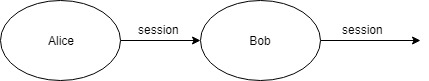
\includegraphics[scale=0.8]{AliceBob.jpg}
%\caption{Forwarding scenario}\label{fig:AliceBob}
%\end{figure}

Let us consider a simple example where a confidential channel $\mathit{session}$ is shared between two parties. %, given in Figure~\ref{fig:AliceBob}. 
Consider that participant $\mathit{Alice}$ is the creator of the channel and that she shares one end-point of the channel with $\mathit{Bob}$. 
The two parties can establish a private interaction over channel $\mathit{session}$, but if $\mathit{Bob}$ forwards his end-point to a third party perhaps $\mathit{Alice}$'s expectation will be frustrated.
%Once the two parties synchronize they can establish a private session over channel $\mathit{session}$.  
%However, after the synchronization, $\mathit{Bob}$ forwards channel $\mathit{session}$ to a third party.

In some cases, it may be appealing to have the forwarding capability. For instance, when a task is forwarded from a master to a slave process, a slave process is a third party and can seamlessly step in.
In our example, this situation may be considered as problematic from the point of view of $\mathit{Alice}$, as she can still believe that the shared end-point of channel $\mathit{session}$, which she may consider confidential, is held by $\mathit{Bob}$. 
If $\mathit{session}$ is a channel created by $\mathit{Alice}$, %possibly 
pointing to some private data %with intention to send some private information along, 
and shared exclusively with $\mathit{Bob}$, %to be the one that access this data, %receives on the other end, 
one might debate that $\mathit{Bob}$ should not acquire the forwarding capability %as $\mathit{Alice}$ 
only by receiving $\mathit{session}$. 
In any case, we can distinguish
two different kinds of channel end-point sharing in the example, as the first one is conducted by the channel creator ($\mathit{Alice}$), while the second can be recognized as forwarding (by $\mathit{Bob}$).

Several formal models have been developed for the purpose of restricting name-sharing considering a statically determined name scope, such as the ones with name grouping~\cite{cardelli05} and name hiding~\cite{Giunti}. 
However, there are cases when there is no statically predefined scope for a piece of private information. For instance, in the example above it may be the case that $\mathit{Alice}$ can decide at some point in the future to share an end-point of $\mathit{session}$ with others. 
In general, we need private information to be shared also in open-ended systems.

Our approach to addressing the problem mentioned above, i.e., to mathematically reason on restricted dissemination of confidential information, is to develop a formal model which disables forwarding directly at the syntax level. Our model, which we name  \emph{Confidential $\pi$-calculus},
 abbreviated $C_\pi$, is a fragment of the $\pi$-calculus~\cite{pi_calculus}. In $C_\pi$ the only resources are channels, and, hence, we treat channel names as confidential information: channels once received cannot be forwarded later on. This is the only difference with respect to the $\pi$-calculus.
 The contribution of the first part of the thesis is the following: 
 \begin{itemize}
 \item  We present a simple fragment of the $\pi$-calculus that allows modeling confidential name passing by restricting forwarding. Being a fragment of a well-established model, such as the $\pi$-calculus, gives us the possibility to directly apply to our model a notable amount of theory already developed.
 \item  We formally characterize the non-forwarding property and, as a sanity check of the process model, we show that all $C_\pi$ processes respect this property.
 \item  Based on the notion of behavioral equivalence relation from the $\pi$-calculus we present a behavioral identity attesting that closed domains for channels can be directly represented in our model.
 \item  We further elaborate on the expressiveness of the $C_\pi$-calculus by showing examples that include closed domains for channels, authentication, and open-ended groups, all of which are also directly represented in the model.
 \item We investigate the expressive power of our model when compared to the $\pi$-calculus and show that the $\pi$-calculus can be encoded into the $C_\pi$-calculus. We show an operational correspondence result for the given encoding.
 \end{itemize}






\section{Access control}\label{sec:intro_access_control}
Another aspect addressed in this thesis is a study of access control in distributed software systems.
The control of access to computational resources is becoming more important, 
despite their availability is growing in scale every year, since such growth encompasses different forms of resource access and raises some issues. 
The need to control access can be motivated by many reasons, such as privacy, security and capacity constraints. 
As examples of capacity constraints consider that physical devices (printers, cell phones, processors, etc.) all have finite capabilities, 
while some virtual devices (shared memory cell, web service, etc.) have infinite potential but their 
availability is frequently limited. 

Privacy and security are central issues in the development of distributed systems. One of the reasons is that distributed systems are nowadays highly complex and heterogeneous, and the access control in such systems can be an error-prone task. Justifications for these claims are appearing almost every day, one of which is the incorrect access token generation on Facebook mentioned previously. For such bad examples companies suffered the loss of millions of dollars, but even worse, privacy and security of millions of users have been compromised. Formal modeling and verification can be a step towards more reliable distributed software systems~\cite{DBLP:journals/jlp/BugliesiCF17}.

%

Various methods for controlling access in distributed systems have been proposed in the past, as the scale and the structure of such systems has been changing.
%
Considering systems that are small or in which the number of participants is predefined, 
access to resources of the system is usually achieved through access control lists (ACL). 
The ACL method uses lists of permissions attached to resources, where the right to access a 
resource is granted only if the user is mentioned as a subject (with the right permission) on 
the access list of the resource.
% 
While the ACL method provides a natural way to control access, when it comes to large-scale systems 
that are highly dynamic this method becomes hard to implement. 
This comes from the fact that access control lists keep information of each user individually, 
which becomes a serious overhead when the number of users of a system is large and frequently changes. 
As an example consider an application, such as Facebook, that is used by millions of users whose number varies over time. 
Having lists of users authorized to access each resource (e.g., pictures or posts of users) becomes arguably impractical. 

Role-based access control method~\cite{sandhu1996role} (RBAC) was introduced as an alternative way 
to deal with the scalability of ACLs. 
In the RBAC method, a set of roles is established and a role is assigned to each user. A user can have more than one role.
For instance, to allow access to a picture of a Facebook user it might not be 
necessary to rely directly on the identity of the user attempting to access the picture. In practice, it is enough to check if the user trying to access 
the picture has the role of a ``friend'' of the owner of the picture. 
%
Besides the advantages (and disadvantages) of the RBAC method with respect to the ACL method, the former still suffers from the fact that there usually must be a central authority that issues and checks the roles of the users.

The capability-based method for access control~\cite{sandhu1994access} is more suitable for uncentralized systems. 
In this method, unforgeable references are created and issued by a central authority, but once issued, these references are held by users. Only when the user wants to access 
the recourse the capability is checked. Hence, a central authority does not have to keep access control information for each user individually, it only checks the validity
of the references when needed, which  significantly reduces the load on central authorities~\cite{zhao2013behavioural}. 
Furthermore, capabilities can be delegated from one user to another without informing the central authority. 
%

Another domain conveying some of the principles of the capability-based access control is 
that of use licenses: a user is allowed to use a software application 
only if it owns a proper license, where we also find an explicit notion of delegation. 
For example, a user, while deploying his 
software application on the cloud computing platform, may delegate his own license, 
potentially losing access to use the application himself, 
a notion known as Bring Your Own License~\cite{byol} (BYOL). 
A specific kind of use licenses, the concurrent use licenses, also provide a flexibility to use the license in a shared way~\cite{baratti2003license}. 
As an example consider a software application that is licensed to be used by an institution. 
In this case, licenses are available to all users in the closed domain of institution, 
but there is a bound on the number of licenses, hence the total number of deployed applications at any point cannot exceed the total number of 
licenses~\cite{license_lp_comp}.

We study capabilities and licenses in an abstract way in
a process model of floating authorizations. 
Authorization is a function determining rights and privileges over a resource.
As before, our focus is on communication centered systems, and hence, 
in our model, the only resources considered are communication channels. 
Thus, an authorization determines the right to use a communication channel. 
A floating authorization in our model represents the right to use a channel in a shared way like in the setting of concurrent use licenses.
In such constellation, we exploit distilled dimensions of floating authorizations: 
domain (to capture where access may be implicitly granted), accounting (to capture the capacity), and delegation (to capture explicit granting).

Our model is an extension of the $\pi$-calculus~\cite{pi_calculus},  
and it builds on previous developments~\cite{DBLP:journals/corr/GhilezanJPPV16, clar:eke}. 
%Hence, our focus is again on communication centered systems.
From the calculus for authorizations of~\cite{DBLP:journals/corr/GhilezanJPPV16} we adopt the syntax constructs for authorization scoping and delegation. 
Semantically, we modify the meaning of authorization scoping construct so as to be able to represent the accounting principle arising from the floating nature of authorizations. Hence, our aim is, therefore, to address  the specific notion of accounting, emerging from the settings of capabilities and licenses, by modifying an existing  model in the minimal necessary way.
%
The contribution of the second part of the thesis is as follows:
\begin{itemize}
\item We present a calculus that models the notions of domain, implicit granting, accounting, and delegation of floating authorizations.  
%
\item We investigate the behavioral semantics of our model: our behavioral characterizations show the specific nature of floating authorizations, in particular, the correlation between the authorization construct and the parallel composition, reflecting our accounting principle. 
%
\item We present a type analysis that singles out processes in which each use of a channel is properly authorized, even in the case of contextual authorizations, and we show type soundness and type safety. 
%
\item We introduce another type system that allows for a more efficient implementation than the original one and we show the respective typing correspondence.
%
\item We give an extended example inspired by the notion of \emph{Bring Your Own License} from the licensing setting.
%
\item Based on the extended example, we show one direction towards the application of our model by considering a possible extension of the Go programming language\footnote{\url{https://golang.org}}.
\end{itemize}





\section{Publications and structure of the thesis}

Controlled name passing is presented in Chapter~\ref{chapter:Cpi}, where we introduce the $C_\pi$-calculus. As noted in Section~\ref{sec:intro_sharing_control}, our calculus models interactions in which information can be shared between two parties, but cannot be forwarded by the receiving party. Chapter~\ref{chapter:Cpi} is based on the paper:
%
\begin{enumerate}
\bibitem{DBLP:journals/corr/abs-1902-0992721}
I.~Proki\'c.
\newblock The {C}pi-calculus: a model for confidential name passing.
\newblock In M.~Bartoletti, L.~Henrio, A.~Mavridou, and A.~Scalas, editors,
  {\em Proceedings 12th Interaction and Concurrency Experience, { ICE 2019}, {
  Copenhagen, Denmark, 20-21 June 2019}}, volume 304 of {\em Electronic
  Proceedings in Theoretical Computer Science}, pages 115--136. Open Publishing
  Association, 2019.
%\bibitem{DBLP:journals/corr/abs-1902-09927}
%I.~Proki{\'c}.
%\newblock The {$C_\pi$}-calculus: a model for confidential name passing.
%\newblock In {\em Interaction and Concurrency Experience, ICE 2019, Held as a
%  Satellite Workshop of the 14th International Federated Conference on
%  Distributed Computing Techniques, DisCoTec 2019, Copenhagen, Denmark, June
%  20-21, 2019}, EPTC, (to appear).
\end{enumerate}
%
The work reported here extends the work presented in the mentioned paper by a more pedagogical introduction of the model and by encompassing all the results. Furthermore, the encoding presented in this document simplifies the one given in the above paper and completes the proof of operational correspondence. 


Controlling resource usages is considered in Chapter~\ref{chapter:auth}, where we introduce our calculus of floating authorizations. Our model allows separating resource awareness from resource usages by authorizations. %: not all parties aware of a resource can use it but only authorized ones. 
Chapter~\ref{chapter:auth} is based on publications:

\begin{enumerate}
%
%
\bibitem{p}
J.~Pantovi{\'c}, I.~Proki{\'c}, and H.~T. Vieira.
\newblock A calculus for modeling floating authorizations.
\newblock In C.~Baier and L.~Caires, editors, {\em Formal Techniques for
  Distributed Objects, Components, and Systems - 38th {IFIP} {WG} 6.1
  International Conference, {FORTE} 2018, Held as Part of the 13th
  International Federated Conference on Distributed Computing Techniques,
  DisCoTec 2018, Madrid, Spain, June 18-21, 2018, Proceedings}, volume 10854 of
  {\em Lecture Notes in Computer Science}, pages 101--120. Springer, 2018.
%
%
\bibitem{PR}
I.~Proki{\'c}, J.~Pantovi{\'c}, and H.~T. Vieira.
\newblock A calculus for modeling floating authorizations.
\newblock {\em Journal of Logical and Algebraic Methods in Programming},
  107:136 -- 174, 2019.
%
%
\end{enumerate}
where the listed journal extends the listed conference publication.

In Chapter~\ref{sec:Conclusions}, we conclude by presenting the contributions of the candidate, providing an overview of the related literature, and, finally, showing some ideas for improvements and possible extensions of the work presented in this thesis.





